% ============================================================
%  BAB 5 – PEMBAHASAN
%  Compile standalone:  pdflatex bab-5.tex
%  Compile as part of thesis: pdflatex main.tex
% ============================================================
\documentclass[main]{subfiles}
\usepackage{hyphenat}
\usepackage{iftex}

% ── Encoding, Language & Fonts ───────────────────────────────
\ifXeTeX
    \usepackage{polyglossia}
    \setmainlanguage{bahasai}
    \usepackage{fontspec}
    \setmainfont{TeX Gyre Termes}
    \setsansfont{TeX Gyre Heros}
    \setmonofont[Scale=0.88]{TeX Gyre Cursor}
\else
    \usepackage[utf8]{inputenc}
    \usepackage[T1]{fontenc}
    \usepackage[indonesian]{babel}
    \usepackage{mathptmx}
    \usepackage{helvet}
    \usepackage{courier}
\fi

% ── Page geometry (A4, UI thesis margins) ────────────────────
\usepackage[
  a4paper,
  top    = 2.54cm,
  bottom = 2.54cm,
  left   = 3.17cm,
  right  = 2.54cm
]{geometry}

% ── Line spacing & paragraph ─────────────────────────────────
\usepackage{setspace}
\onehalfspacing
\setlength{\parindent}{1.27cm}
\setlength{\parskip}{0pt}

% ── Microtype & justification ────────────────────────────────
\usepackage{microtype}
\sloppy

% ── Headings ─────────────────────────────────────────────────
\usepackage{titlesec}

\titleformat{\chapter}[block]
  {\centering\sffamily\bfseries\large}{}
  {0pt}{\MakeUppercase}
\titlespacing*{\chapter}{0pt}{0pt}{1.5em}

\titleformat{\section}
  {\sffamily\bfseries\normalsize}{\thesection}{1em}{}
\titlespacing*{\section}{0pt}{1.2em}{0.6em}

\titleformat{\subsection}
  {\sffamily\bfseries\normalsize}{\thesubsection}{1em}{}
\titlespacing*{\subsection}{0pt}{1em}{0.5em}

\titleformat{\subsubsection}
  {\sffamily\bfseries\normalsize}{\thesubsubsection}{1em}{}
\titlespacing*{\subsubsection}{0pt}{0.8em}{0.4em}

% ── Tables ───────────────────────────────────────────────────
\usepackage{longtable, booktabs, array, multirow}
\usepackage{calc}
\usepackage{tabularx}

% ── Math ─────────────────────────────────────────────────────
\usepackage{amsmath, amssymb}

% ── Graphics ─────────────────────────────────────────────────
\usepackage{graphicx}
\makeatletter
\def\maxwidth{\ifdim\Gin@nat@width>\linewidth\linewidth\else\Gin@nat@width\fi}
\makeatother
\setkeys{Gin}{width=\maxwidth,keepaspectratio}

% ── Lists ────────────────────────────────────────────────────
\usepackage{enumitem}
\setlist[enumerate,1]{
  label      = \arabic*.,
  leftmargin = 1.27cm,
  itemsep    = 4pt,
  parsep     = 0pt,
  topsep     = 4pt
}
\setlist[enumerate,2]{
  label      = \alph*.,
  leftmargin = 1.27cm,
  itemsep    = 3pt,
  parsep     = 0pt,
  topsep     = 2pt
}

% ── Hyperlinks ───────────────────────────────────────────────
\usepackage[hidelinks]{hyperref}

% Bibliography setup is inherited from main.tex (biblatex + references.bib)
% when this file is compiled standalone via the subfiles class.

% ============================================================
\begin{document}

% When standalone: set counter so \chapter{} renders as "BAB 5".
% When in main.tex: main.tex sets the counter before \subfile{bab-5}.
\ifSubfilesClassLoaded{}{\setcounter{chapter}{4}}

\chapter{Pembahasan}\label{sec:hasil-evaluasi}

Bab ini memaparkan hasil evaluasi atas artefak yang dikembangkan pada bab
sebelumnya beserta pembahasannya. Dalam kerangka \textit{Design Science
Research} (DSR), tahap
evaluasi bertujuan mengukur performa dan kualitas \textit{Knowledge Graph}
(KG) yang dihasilkan oleh \textit{pipeline} sistem. Evaluasi dilakukan secara
komprehensif melalui analisis kuantitatif terhadap topologi graf,
validasi kualitatif oleh pakar domain, pembahasan mendalam terkait
\textit{error} model LLM, serta komparasi antar-disiplin ilmu sains.

% ────────────────────────────────────────────────────────────
\section{Hasil Analisis Struktural Graf}\label{subsec:struktural}
% ────────────────────────────────────────────────────────────

Analisis struktural bertujuan untuk mengevaluasi kualitas interkoneksi
jaringan pengetahuan secara matematis, khususnya untuk melihat
perbandingan struktur graf sebelum \textit{Knowledge Graph Completion} (pre-KGC)
dan sesudahnya (post-KGC). Seluruh perhitungan pada bagian ini
dieksekusi melalui kueri \textit{Cypher} di Neo4j dengan berpedoman pada
formulasi metrik topologi yang telah dijelaskan pada Subbab~\ref{subsec:metrik-topologi}.
Perbandingan topologi graf sebelum dan sesudah KGC ditunjukkan pada
Gambar~\ref{fig:kg-topologi}: pada kondisi pra-KGC tampak tiga graf
yang terpisah, mencerminkan ketiga komunitas mata pelajaran yang
terisolasi, sedangkan pada kondisi pasca-KGC ketiga graf tersebut saling
terhubung oleh relasi lintas-buku.

\begin{figure}[htbp]
  \centering
  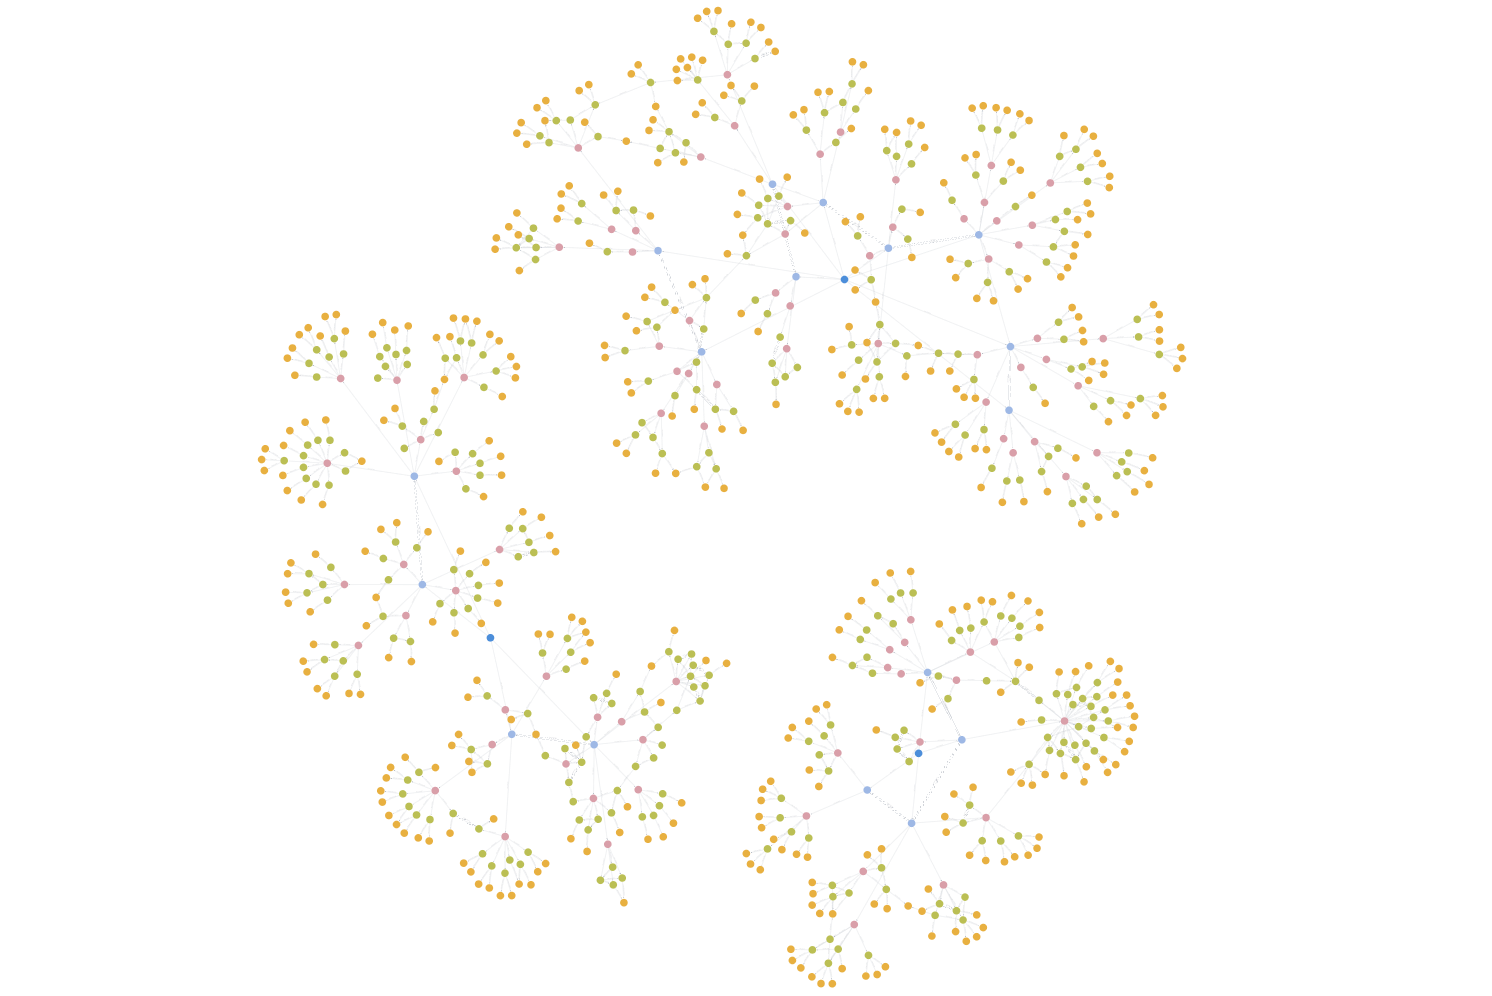
\includegraphics[width=0.82\linewidth]{figures/kg/pre-kgc.png}\\[0.2em]
  {\small (a) Pra-KGC}\\[0.8em]
  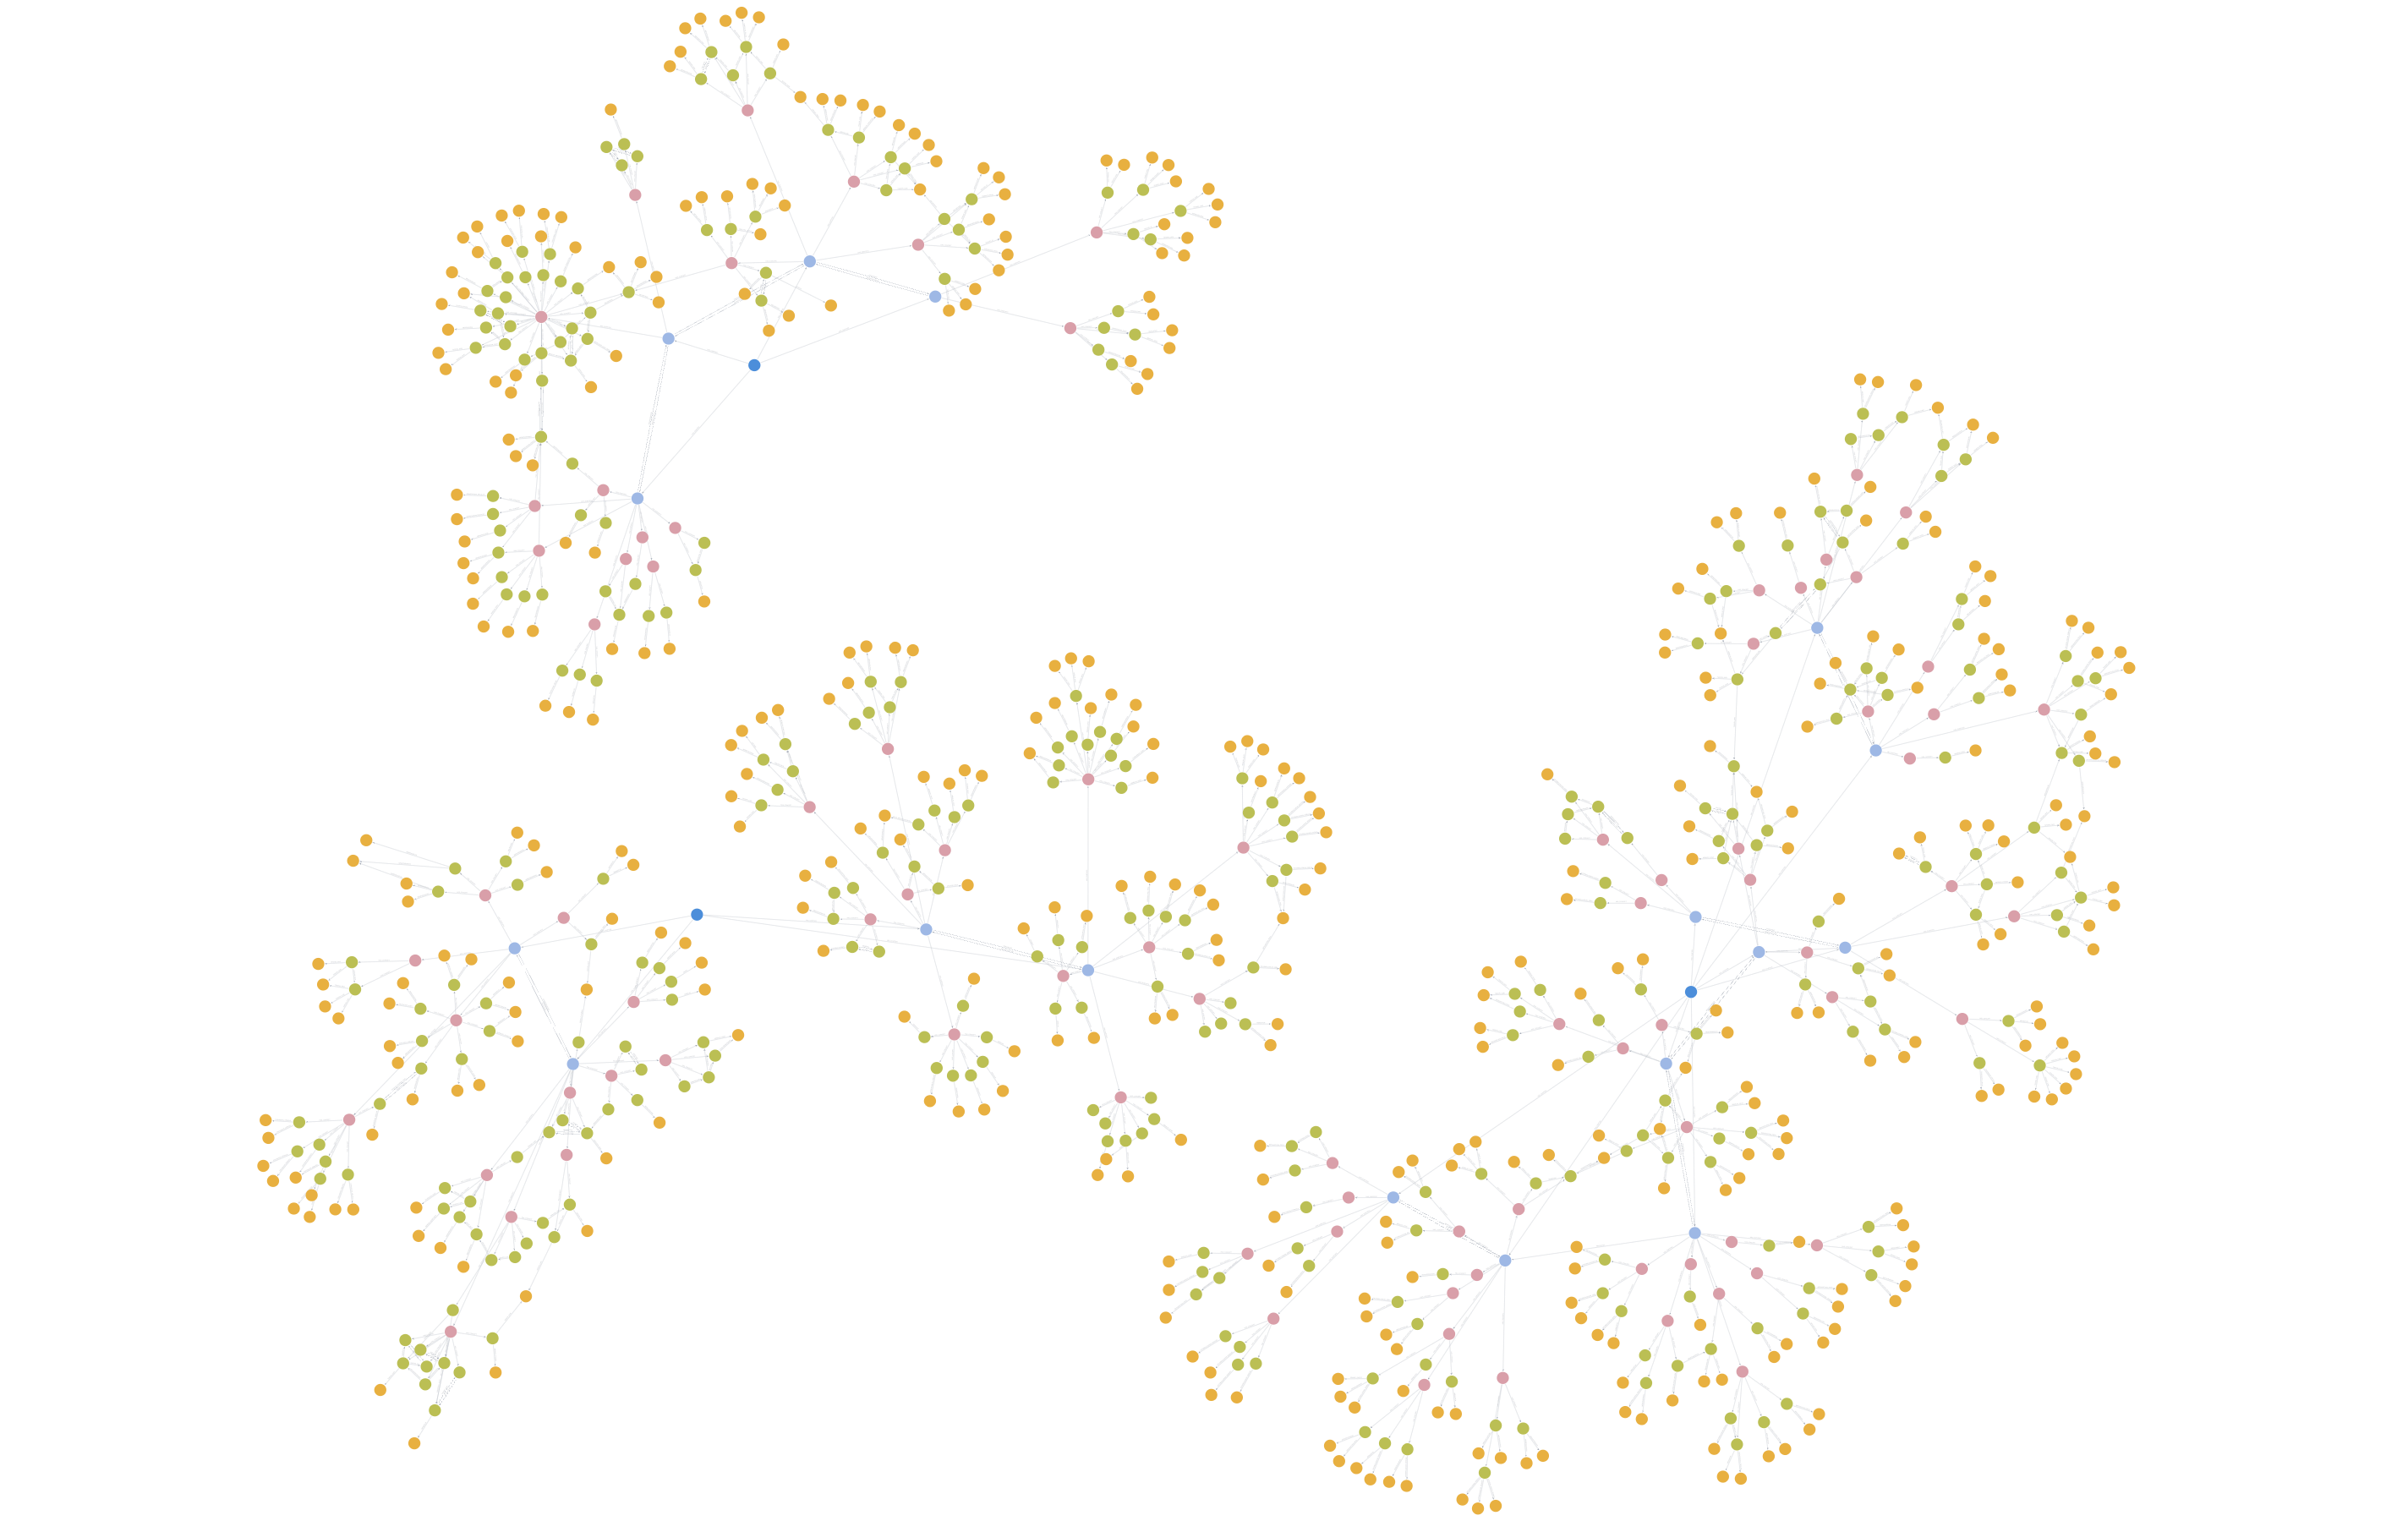
\includegraphics[width=0.82\linewidth]{figures/kg/post-kgc.png}\\[0.2em]
  {\small (b) Pasca-KGC}
  \caption{Perbandingan topologi \textit{knowledge graph} sebelum (a) dan
    sesudah (b) proses KGC. Penambahan relasi lintas-buku menjembatani
    ketiga komunitas mata pelajaran yang semula terpisah.}
  \label{fig:kg-topologi}
\end{figure}

\begin{longtable}{@{}
  >{\raggedright\arraybackslash}p{0.38\linewidth}
  >{\centering\arraybackslash}p{0.27\linewidth}
  >{\centering\arraybackslash}p{0.27\linewidth}@{}}
\caption{Perbandingan metrik struktural pre-KGC dan post-KGC.}
\label{tab:struktural}\\
\toprule
\textbf{Metrik Struktural} & \textbf{Pre-KGC} & \textbf{Post-KGC} \\
\midrule
\endhead
ADC (seluruh node)                & 2{,}4123 & 2{,}6970 \\
ADC (Konsep-ke-Konsep)            & 0{,}7384 & 1{,}4651 \\
\textit{Graph Density} (antar-konsep) & 0{,}00108 & 0{,}00214 \\
\textit{Modularity}               & 0{,}8106 & 0{,}3732 \\
\bottomrule
\end{longtable}

\begin{enumerate}
  \item \textbf{Evaluasi \textit{Average Degree Centrality} (ADC) dan Kepadatan.}

  Berdasarkan Tabel~\ref{tab:struktural}, ADC seluruh node meningkat dari 2{,}41
  (pre-KGC) menjadi 2{,}70 (post-KGC), kenaikan sebesar 11{,}8\%. Namun
  peningkatan yang lebih signifikan terjadi pada ADC Konsep-ke-Konsep, yang hampir
  berlipat ganda dari 0{,}74 menjadi 1{,}47 (+98{,}4\%). Peningkatan ini
  mencerminkan bahwa \textit{pipeline} KGC berhasil menambahkan 125 relasi
  lintas-buku baru yang secara langsung menghubungkan node Concept antar-mapel,
  meningkatkan kepadatan interkoneksi semantik yang sebelumnya tidak ada.
  \textit{Graph Density} antar-konsep, yakni kepadatan relasi pada subgraf
  \texttt{Concept} (lihat Subbab~\ref{subsec:metrik-topologi}), juga meningkat
  secara proporsional dari 0{,}00108 menjadi 0{,}00214 (hampir dua kali lipat),
  konsisten dengan penambahan \textit{edge} lintas-buku tersebut. Nilai densitas
  yang masih sangat rendah pada kedua fase merupakan karakteristik umum
  \textit{knowledge graph} berukuran sedang-besar, karena hanya sebagian kecil
  dari seluruh kemungkinan pasangan konsep yang memiliki relasi bermakna
  \parencite{hogan_knowledge_2022}.

  \item \textbf{Evaluasi \textit{Modularity}.}

  \textit{Modularity} di sini dihitung atas partisi komunitas \textbf{tetap}
  berdasarkan mata pelajaran (Fisika, Kimia, Biologi), sesuai dengan
  formulasi pada Subbab~\ref{subsec:metrik-topologi}. Dengan demikian, perubahan
  nilai $Q$ murni mencerminkan bertambahnya \textit{edge} lintas-mapel.
  Analisis struktur komunitas menggunakan metrik \textit{Modularity} pada fase
  pre-KGC mencatatkan nilai 0{,}811, yang mengindikasikan struktur komunitas yang
  sangat kuat --- ketiga komunitas mapel (Fisika, Kimia, Biologi) hampir sepenuhnya
  terisolasi satu sama lain, sejalan dengan kondisi \textit{siloed learning} yang
  diidentifikasi sebagai masalah penelitian. Setelah KGC, nilai \textit{Modularity}
  turun secara signifikan menjadi 0{,}373, menandakan bahwa relasi lintas-buku yang
  ditambahkan berhasil menjembatani ketiga komunitas tersebut dan mengurangi
  keterpisahan topologis antar-disiplin. Penurunan ini merupakan indikator
  keberhasilan utama \textit{pipeline}, karena penurunan \textit{Modularity}
  mencerminkan peningkatan interkoneksi lintas-komunitas sebagaimana dirumuskan
  pada Subbab~\ref{subsec:metrik-topologi}.

  \item \textbf{Evaluasi Metrik Ekstraksi dan Hubungan.}

  Di luar evaluasi topologi di atas, kualitas hasil ekstraksi LLM secara
  spesifik diukur menggunakan metrik \textit{Description Completeness} (DC),
  \textit{Empty SubKonsep Rate} (ESR), dan
  \textit{Typed Relation Ratio} (TRR) sebagaimana didefinisikan pada
  Subbab~\ref{subsec:metrik-ekstraksi} dan~\ref{subsec:metrik-hubungan}.
  Sistem mencatatkan nilai DC sebesar 93{,}07\% --- identik pada
  fase pre-KGC maupun post-KGC karena DC mengukur kualitas deskripsi node yang
  tidak berubah akibat penambahan \textit{edge} KGC. Metrik ESR tercatat 0\%
  (0,00) pada kedua fase --- jauh di bawah ambang maksimal 10\% --- yang
  menandakan bahwa seluruh entitas induk (\texttt{:Subtopic}) berhasil
  didekomposisi menjadi setidaknya satu konsep turunan, sehingga tidak ada
  ``node buntu'' dalam graf. Nilai TRR meningkat dari
  69{,}69\% (pre-KGC) menjadi 74{,}86\% (post-KGC), mencerminkan bahwa KGC
  menambahkan \textit{edge} bertipe semantik spesifik sehingga proporsi relasi
  bertype meningkat relatif terhadap total \textit{edge} dalam graf.
\end{enumerate}

% ────────────────────────────────────────────────────────────
\section{Hasil Validasi Pakar}\label{subsec:validasi-pakar}
% ────────────────────────────────────────────────────────────

Performa sistem dalam mengekstrak dan memprediksi relasi dinilai langsung oleh
panel enam pakar menggunakan instrumen KG Review App. Sesuai desain studi dua
fase, hasil penilaian dipisahkan menjadi validasi intra-mapel (Fase 1) dan
inter-mapel (Fase 2). Data dianalisis menggunakan metrik \textit{Precision},
\textit{Recall}, dan F1-Score, serta uji kesepakatan Gwet's AC1, sebagaimana
didefinisikan pada Subbab~\ref{subsec:validasi-manusia}.

{\setlength{\tabcolsep}{3pt}
\begin{longtable}{@{}
  >{\raggedright\arraybackslash}p{0.13\linewidth}
  >{\raggedright\arraybackslash}p{0.12\linewidth}
  >{\centering\arraybackslash}p{0.085\linewidth}
  >{\centering\arraybackslash}p{0.075\linewidth}
  >{\centering\arraybackslash}p{0.075\linewidth}
  >{\centering\arraybackslash}p{0.055\linewidth}
  >{\centering\arraybackslash}p{0.065\linewidth}
  >{\centering\arraybackslash}p{0.07\linewidth}
  >{\centering\arraybackslash}p{0.07\linewidth}@{}}
\caption{Hasil validasi Fase 1 (intra-mapel) per penilai dan konsensus final.
  Baris ``Final'' merupakan label konsensus setelah resolusi ketidaksepakatan
  via \textit{LLM-as-a-judge}. Presisi (P) dihitung sebagai \textit{Fuzzy
  Precision} dengan bobot Benar $=1{,}0$, Parsial (Sebagian Benar) $=0{,}5$,
  Kurang Konteks (KK) $=0{,}25$, dan Salah $=0$; seluruh \textit{triple} yang
  ditinjau tetap masuk ke dalam penyebut presisi. 
  Selisih jumlah ``Ditinjau'' antara baris Final dan baris penilai
  berasal dari sejumlah kecil \textit{triple} yang dikonsolidasikan dan
  dikeluarkan dari himpunan evaluasi saat penentuan konsensus.}
\label{tab:validasi-mapel}\\
\toprule
\textbf{Mapel} & \textbf{Penilai} & \textbf{Ditinjau} & \textbf{Benar} & \textbf{Parsial} & \textbf{KK} & \textbf{Salah} & \textbf{P} & \textbf{R} \\
\midrule
\endhead
Biologi  & Expert 1      & 151 & 140 & 6  & 3  & 2  & 0{,}952 & 0{,}965 \\
         & Expert 2      & 151 & 143 & 6  & 2  & 0  & 0{,}970 & 0{,}970 \\
         & \textit{Final}& 151 & 144 & 4  & 2  & 1  & \textbf{0{,}970} & \textbf{0{,}977} \\
\midrule
Fisika   & Expert 1      & 240 & 239 & 0  & 1  & 0  & 0{,}997 & 0{,}938 \\
         & Expert 2      & 240 & 186 & 40 & 11 & 3  & 0{,}870 & 0{,}881 \\
         & \textit{Final}& 235 & 215 & 18 & 0  & 2  & \textbf{0{,}953} & \textbf{0{,}922} \\
\midrule
Kimia    & Expert 1      & 166 & 132 & 7  & 2  & 25 & 0{,}819 & 0{,}965 \\
         & Expert 2      & 166 & 136 & 6  & 19 & 5  & 0{,}866 & 0{,}757 \\
         & \textit{Final}& 158 & 135 & 6  & 2  & 15 & \textbf{0{,}877} & \textbf{0{,}855} \\
\midrule
Keseluruhan & Expert 1   & 557 & 511 & 13 & 6  & 27 & 0{,}932 & 0{,}952 \\
            & Expert 2   & 557 & 465 & 52 & 32 & 8  & 0{,}896 & 0{,}863 \\
            & \textit{Final} & 544 & 494 & 28 & 4 & 18 & \textbf{0{,}936} & \textbf{0{,}917} \\
\bottomrule
\end{longtable}
}

\begin{longtable}{@{}
  >{\raggedright\arraybackslash}p{0.18\linewidth}
  >{\centering\arraybackslash}p{0.14\linewidth}
  >{\centering\arraybackslash}p{0.14\linewidth}
  >{\centering\arraybackslash}p{0.14\linewidth}
  >{\centering\arraybackslash}p{0.14\linewidth}
  >{\centering\arraybackslash}p{0.14\linewidth}@{}}
\caption{Uji kesepakatan antar-penilai Gwet's AC1 per mata pelajaran (Fase 1).}
\label{tab:ac1}\\
\toprule
\textbf{Mapel} & \textbf{Item} & \textbf{Obs. Agreement} & \textbf{Chance Agr.} & \textbf{Gwet's AC1} & \textbf{Interpretasi} \\
\midrule
\endhead
Biologi & 151 & 0{,}934 & 0{,}040 & \textbf{0{,}931} & Sangat tinggi \\
Fisika  & 240 & 0{,}771 & 0{,}069 & \textbf{0{,}754} & Substansial \\
Kimia   & 166 & 0{,}651 & 0{,}112 & \textbf{0{,}607} & Moderat \\
\bottomrule
\end{longtable}

\begin{longtable}{@{}
  >{\raggedright\arraybackslash}p{0.20\linewidth}
  >{\centering\arraybackslash}p{0.18\linewidth}
  >{\centering\arraybackslash}p{0.18\linewidth}
  >{\centering\arraybackslash}p{0.18\linewidth}
  >{\centering\arraybackslash}p{0.18\linewidth}@{}}
\caption{Ringkasan metrik per fase evaluasi. Fase 2: kolom Precision melaporkan validitas relasi (116/117); Recall dan F1 tidak dapat dihitung (tidak ada data \textit{missing triples}); AC1 tidak berlaku (panel diskusi tunggal).}
\label{tab:validasi-metrik}\\
\toprule
\textbf{Fase} & \textbf{Precision} & \textbf{Recall} & \textbf{F1-Score} & \textbf{Gwet's AC1} \\
\midrule
\endhead
Fase 1 (konsensus) & 0{,}936 & 0{,}917 & 0{,}926 & lihat Tabel~\ref{tab:ac1} \\
Fase 2 (panel diskusi) & 0{,}991 & — & — & — \\
\bottomrule
\end{longtable}

\begin{enumerate}
  \item \textbf{Kuantitas Akurasi (Precision, Recall, F1-Score).}

  Secara agregat pada Fase 1, \textit{precision} konsensus final mencapai 93{,}6\%
  dan \textit{recall} 91{,}7\%, menghasilkan F1-Score sebesar 92{,}6\%
  (Tabel~\ref{tab:validasi-mapel}). Nilai ini menunjukkan bahwa
  kemampuan LLM dalam mengekstraksi relasi intra-mapel tergolong baik. Biologi
  mencatatkan F1 tertinggi (0{,}973), diikuti Fisika (0{,}937), dan Kimia (0{,}866).

  Pada level keseluruhan, \textit{precision} melampaui \textit{recall} sebesar
  1{,}9 poin. Selisih ini melebar pada konsensus final Fisika (3{,}1 poin) dan
  terutama pada penilaian Expert 2 Kimia (10{,}9 poin). Penyebab utamanya adalah
  \textit{missing triples} (10 relasi pada konsensus final Fisika dan 29 relasi
  yang dilaporkan Expert 2 Kimia) yang menandakan sistem masih luput
  mengekstrak sebagian relasi kuantitatif dan terminologi proses yang esensial.
  Perbedaan standar antar penilai juga tampak jelas pada Fisika (Expert 1 vs.\
  Expert 2: P 0{,}997 vs.\ 0{,}870; R 0{,}938 vs.\ 0{,}881), dan dikonfirmasi
  oleh nilai AC1 Fisika yang tergolong moderat (0{,}754).

  Pada Fase 2 (inter-mapel), validasi panel diskusi atas 117 relasi lintas-buku
  menghasilkan \textit{precision} (validitas) 99{,}1\% (116/117 relasi dikonfirmasi
  valid; satu relasi ditolak). Metrik \textit{Recall} dan F1 tidak dapat dihitung
  karena tidak tersedia informasi jumlah total relasi lintas-buku yang benar
  (denominator \textit{recall}) dalam konfigurasi panel tunggal ini. Karena validasi
  dilakukan melalui diskusi panel (bukan dua penilai independen), uji Gwet's AC1
  tidak berlaku.

  \item \textbf{Uji Kesepakatan Pakar (Inter-rater Reliability).}

  Sesuai dengan pilihan metodologi yang ditetapkan pada Bab 3 (dan latar belakang
  teoritis Gwet's AC1 pada Subbab~\ref{subsec:validasi-manusia}), uji kesepakatan antar-pakar menggunakan
  Gwet's AC1. Hasil pada Tabel~\ref{tab:ac1} menunjukkan variasi tingkat kesepakatan
  yang signifikan antar mata pelajaran. Biologi mencatatkan AC1 tertinggi (0{,}931),
  mengindikasikan kesepakatan yang hampir sempurna antara kedua penilai. Hal ini
  konsisten dengan sifat konten Biologi yang lebih deskriptif dan definitif. Fisika
  memperoleh AC1 substansial (0{,}754), sedangkan Kimia mencatatkan AC1 moderat
  (0{,}607). Nilai AC1 Kimia yang paling rendah selaras dengan pola kesalahan pada
  Subbab~\ref{subsubsec:error-analysis}: terminologi proses kimia (seperti elektrorefining vs.\
  electroplating) memiliki batas semantik yang lebih ambigu, sehingga kedua penilai
  lebih sering tidak sepakat.
\end{enumerate}

% ────────────────────────────────────────────────────────────
\section{Pembahasan Kualitatif Hasil KGC}\label{subsec:kualitatif}
% ────────────────────────────────────────────────────────────

Bagian ini membahas secara kualitatif kualitas relasi lintas-buku yang
ditemukan oleh \textit{pipeline Graph Completion}, menganalisis pola kesalahan
model LLM, dan mengidentifikasi faktor-faktor yang memengaruhi akurasi
ekstraksi.

Pengaruh parameter \textit{retrieval} terhadap jumlah relasi lintas-buku yang
ditemukan dievaluasi pada empat konfigurasi berpasangan (Tabel~\ref{tab:param-sweep});
ambang kemiripan (\textit{threshold}) dinaikkan seiring penurunan jumlah
tetangga per node (top-$k$). Semakin ketat konfigurasi, semakin sedikit pasangan
kandidat yang lolos: dari 125 relasi pada konfigurasi paling permisif (0{,}70
/ top-$k$ = 20) menyusut menjadi hanya 14 relasi pada konfigurasi paling ketat
(0{,}85 / top-$k$ = 5). Analisis kualitas per konfigurasi disajikan pada
Subbab~\ref{subsubsec:kualitas}.

\begin{figure}[htbp]
  \centering
  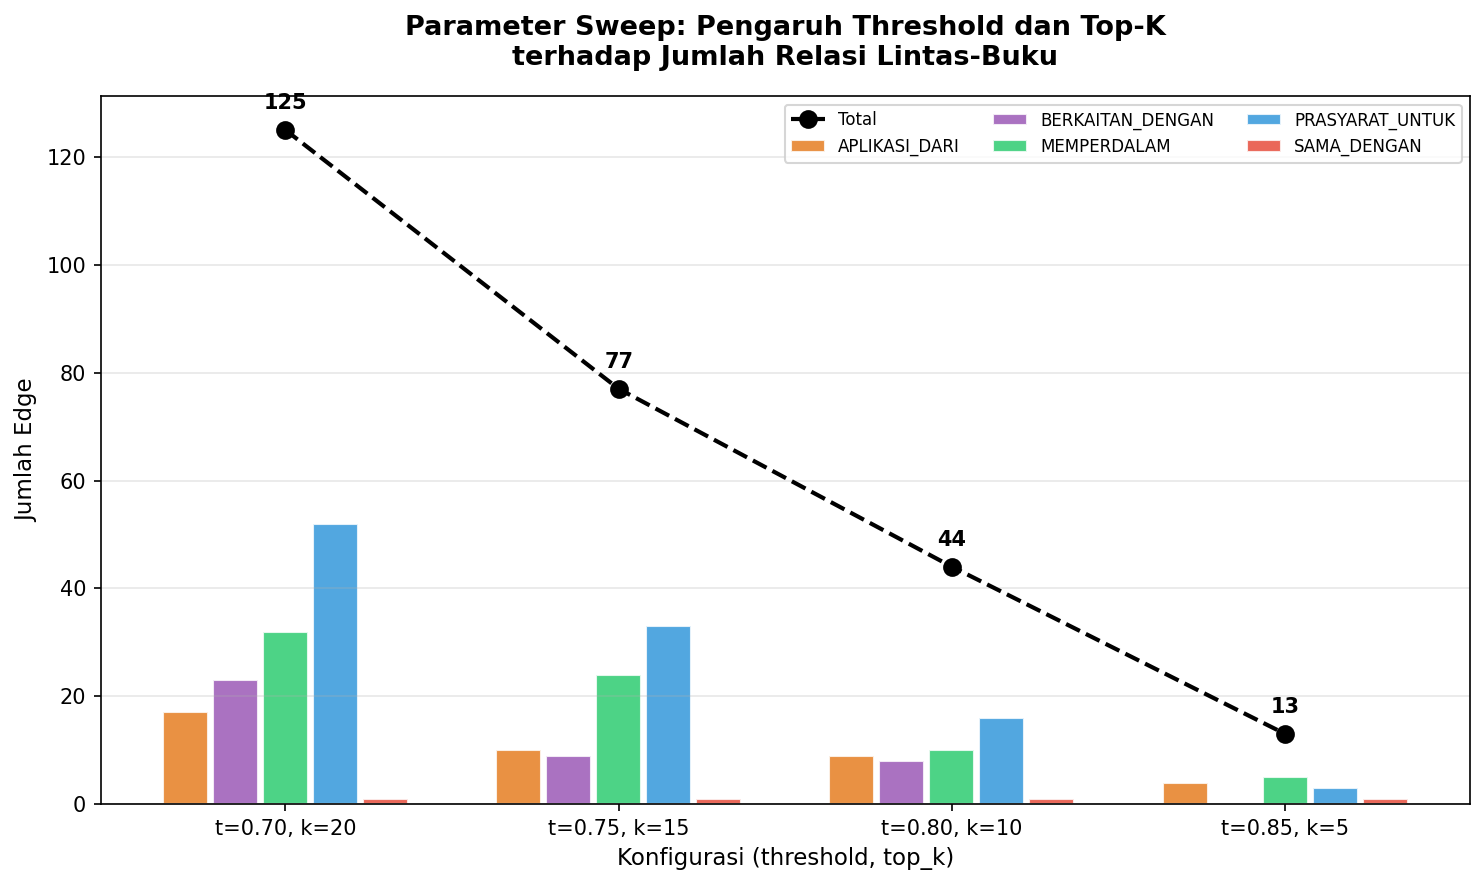
\includegraphics[width=\maxwidth]{images/media/image3.png}
  \caption{\textit{Parameter sweep}: pengaruh \textit{threshold} dan top-$k$ terhadap
    jumlah relasi lintas-buku yang ditemukan.}
  \label{fig:param-sweep}
\end{figure}

\begin{longtable}{@{}
  >{\raggedright\arraybackslash}p{0.40\linewidth}
  >{\raggedright\arraybackslash}p{0.54\linewidth}@{}}
\caption{Jumlah relasi lintas-buku per konfigurasi \textit{parameter sweep}.}
\label{tab:param-sweep}\\
\toprule
\textbf{Konfigurasi (threshold / top-$k$)} & \textbf{Jumlah relasi} \\
\midrule
\endhead
0{,}70 / $k$=20 (permisif --- konfigurasi final) & 125 \\
0{,}75 / $k$=15                                   & 72  \\
0{,}80 / $k$=10                                   & 42  \\
0{,}85 / $k$=5 (paling ketat)                     & 14  \\
\bottomrule
\end{longtable}

\begin{figure}[htbp]
  \centering
  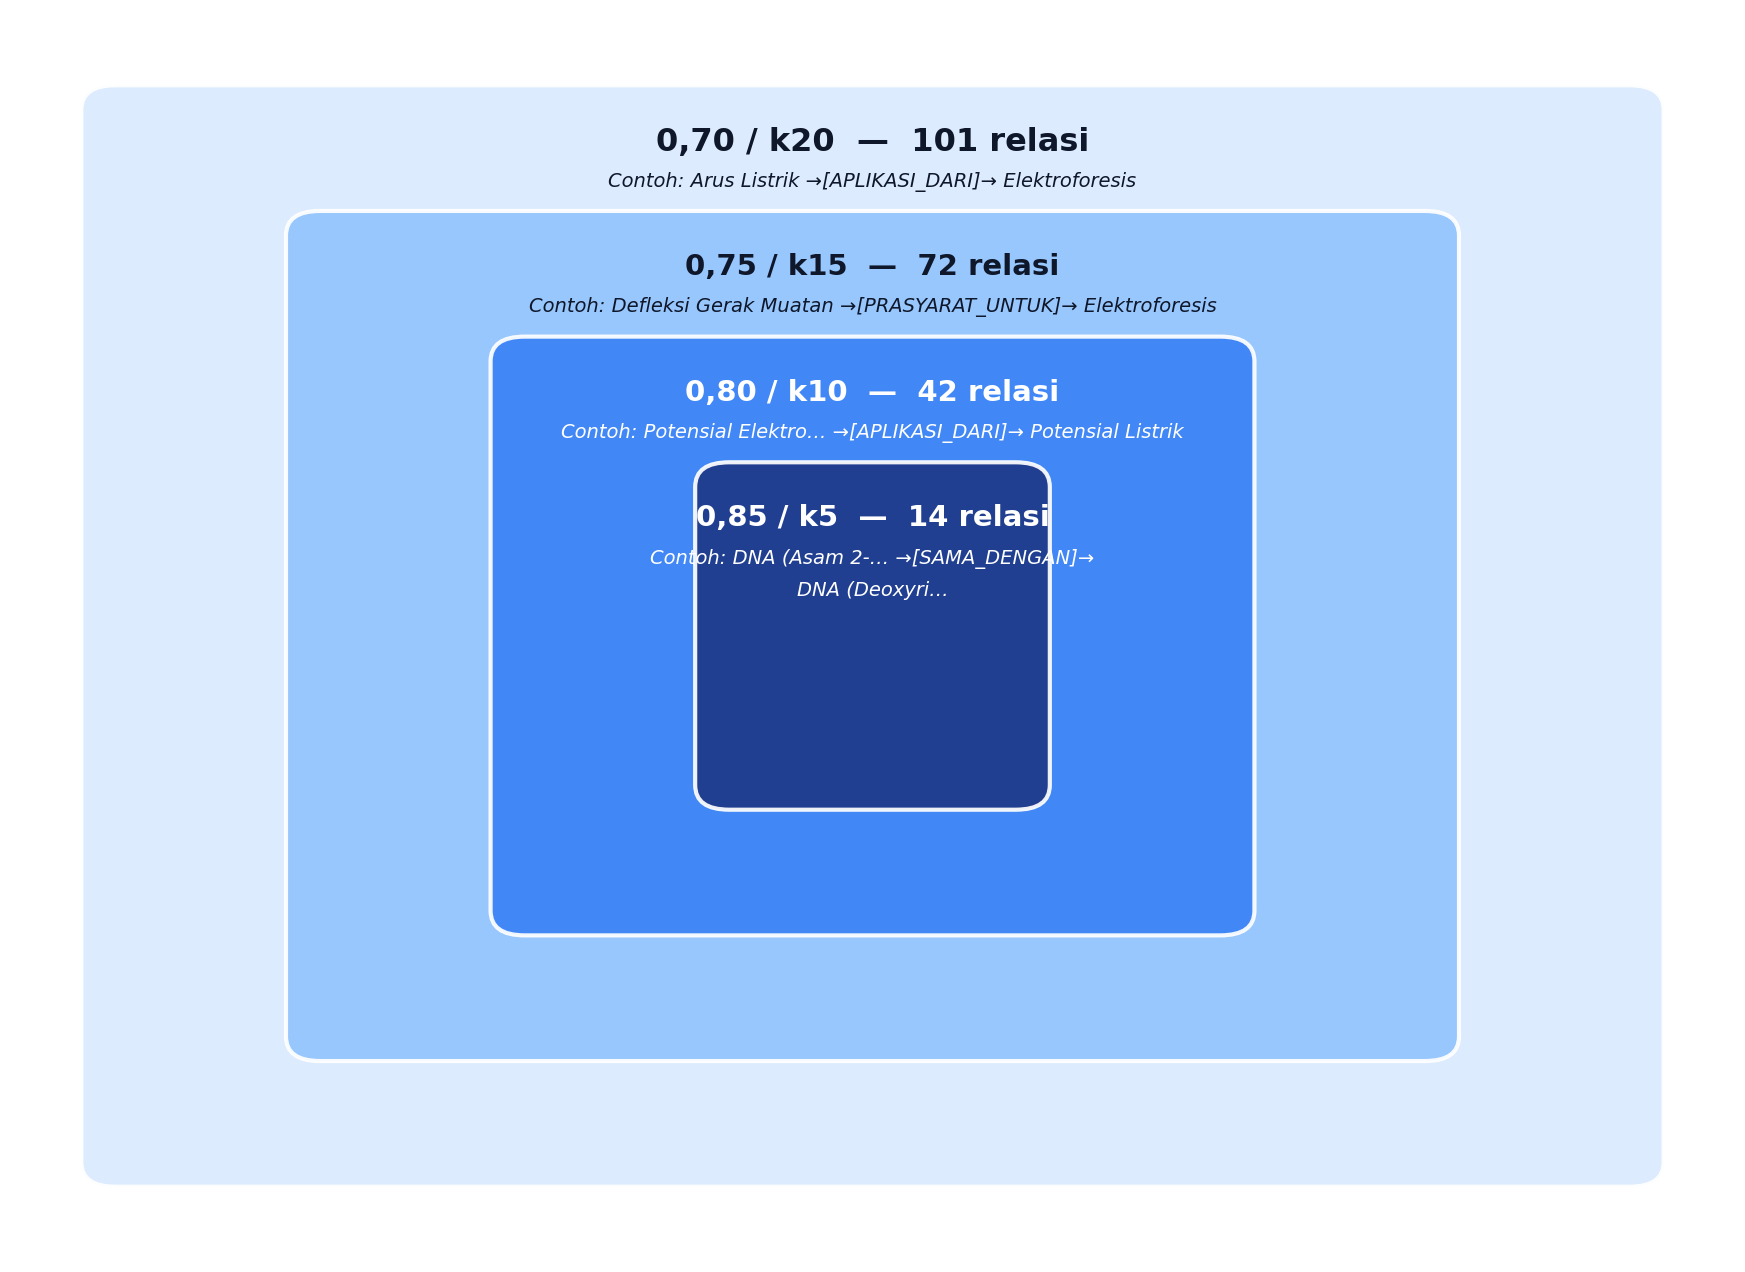
\includegraphics[width=\maxwidth]{images/media/image4.png}
  \caption{Struktur bersarang (\textit{nested}) hasil \textit{parameter sweep} relasi
    lintas-buku. Setiap konfigurasi yang lebih ketat merupakan himpunan bagian
    (\textit{subset}) dari konfigurasi yang lebih permisif.}
  \label{fig:nested-sweep}
\end{figure}

Konfigurasi membentuk himpunan bersarang: setiap konfigurasi yang lebih
ketat merupakan himpunan bagian dari yang lebih permisif. Pengetatan
parameter dengan demikian berfungsi sebagai kompromi \textit{recall} ---
menukar cakupan relasi (lebih banyak interkoneksi ditemukan) dengan
selektivitas (hanya pasangan berkemiripan tertinggi yang dipertahankan).
Sebagaimana akan dibahas pada Subbab~\ref{subsubsec:kualitas}, pengetatan ini menurunkan
kuantitas relasi tetapi \textbf{tidak} memperbaiki ketepatan arah relasi.

% ──────────────────────────────────────────
\subsection{Kualitas Relasi Lintas-Buku yang Ditemukan}\label{subsubsec:kualitas}
% ──────────────────────────────────────────

Pada konfigurasi final (threshold = 0{,}70; top-$k$ = 20; \textit{scope}
lintas-mapel), \textit{pipeline} menemukan 125 relasi lintas-buku. Distribusi
tipe relasi (Gambar~\ref{fig:relasi-distribusi}) didominasi PRASYARAT\_UNTUK (57 \textit{edge}, 45{,}6\%), diikuti
MEMPERDALAM (31 \textit{edge}, 24{,}8\%), BERKAITAN\_DENGAN (21 \textit{edge}, 16{,}8\%),
APLIKASI\_DARI (15 \textit{edge}, 12{,}0\%), dan SAMA\_DENGAN (1 \textit{edge}, 0{,}8\%).
Dominasi PRASYARAT\_UNTUK mengindikasikan bahwa jembatan lintas-disiplin
pada kurikulum sains kelas XII lebih banyak bersifat prasyarat pengetahuan
daripada aplikasi atau analogi. Dari 125 relasi, 8 \textit{edge} memiliki \textit{confidence}
$< 0{,}5$ (seluruhnya BERKAITAN\_DENGAN) dikeluarkan dari survei validasi
utama, menyisakan 117 relasi yang dinilai pakar.

\begin{figure}[htbp]
  \centering
  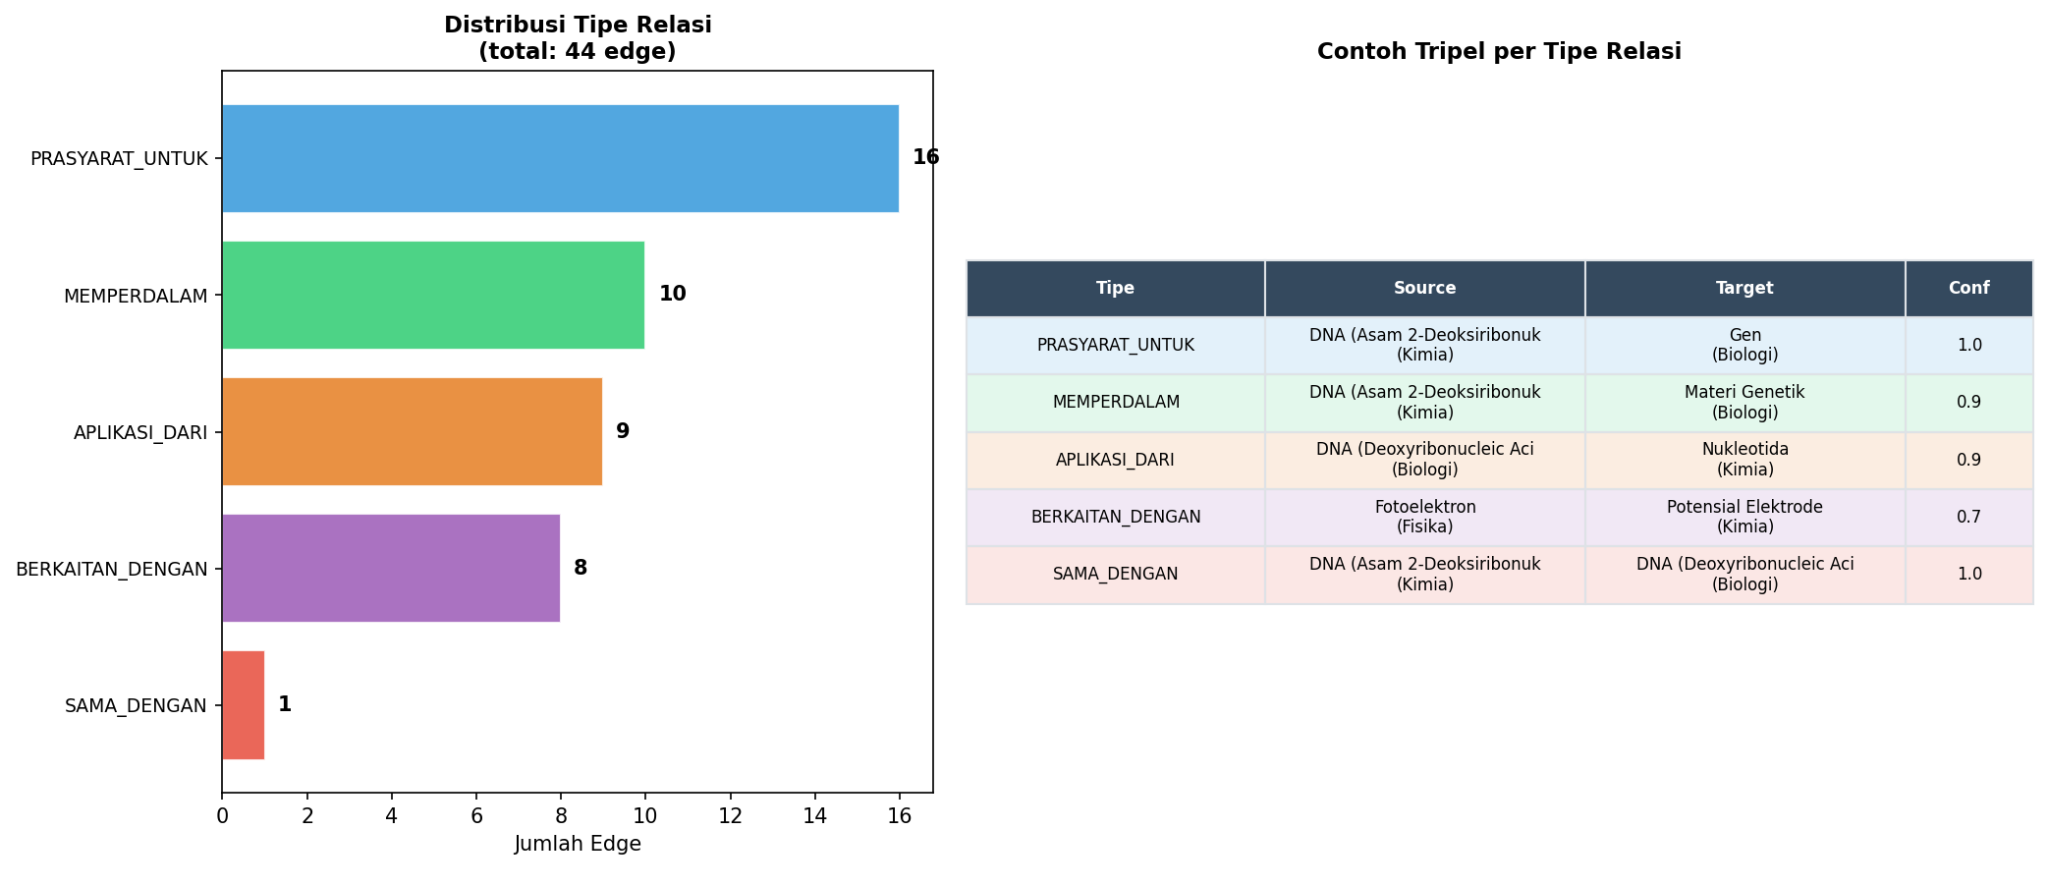
\includegraphics[width=\maxwidth]{images/media/image22.png}
  \caption{Distribusi tipe relasi lintas-buku hasil klasifikasi LLM beserta contoh triple per tipe.}
  \label{fig:relasi-distribusi}
\end{figure}

Dari 125 \textit{edge}, 20 (16\%) memiliki skor \textit{confidence} = 1{,}0, menunjukkan
keyakinan tinggi LLM terhadap relasi tersebut. Contoh relasi dengan
\textit{confidence} tertinggi meliputi:

\begin{itemize}
  \item DNA (Asam 2-Deoksiribonukleat) [Kimia] $\to$ Gen [Biologi]:
    PRASYARAT\_UNTUK (conf = 1{,}0). Pemahaman struktur kimia DNA merupakan
    fondasi untuk memahami fungsi gen secara biologis.
  \item Potensial Elektrode [Kimia] $\to$ Potensial Listrik [Fisika]:
    APLIKASI\_DARI (conf = 1{,}0). Konsep potensial elektrode dalam
    elektrokimia merupakan aplikasi langsung dari konsep potensial listrik
    dalam fisika.
  \item Enzim [Biologi] $\to$ Protein [Kimia]: APLIKASI\_DARI (conf = 1{,}0).
    Enzim merupakan manifestasi fungsional dari protein dalam konteks biologis.
  \item Fosforilasi Oksidatif [Biologi] $\to$ Oksidasi [Kimia]:
    PRASYARAT\_UNTUK (conf = 1{,}0). Pemahaman reaksi oksidasi secara kimia
    diperlukan sebelum mempelajari fosforilasi oksidatif dalam metabolisme.
\end{itemize}

Satu-satunya relasi bertipe SAMA\_DENGAN yang ditemukan adalah DNA (Asam
2-Deoksiribonukleat) [Kimia] $\leftrightarrow$ DNA (Deoxyribonucleic Acid)
[Biologi] dengan \textit{confidence} 1{,}0. Temuan ini mengonfirmasi bahwa
\textit{pipeline} mampu mendeteksi entitas identik yang diajarkan di dua disiplin
berbeda dengan terminologi yang sedikit berbeda.

\subsubsection{Validasi Pakar atas Relasi Lintas-Buku}

Seluruh 117 relasi kandidat pada konfigurasi final ($\tau$=0{,}70, $k$=20)
divalidasi pakar melalui instrumen survei Fase~2 yang menilai validitas,
ketepatan tipe, dan ketepatan arah tiap relasi secara \textit{score-blind}
melalui diskusi panel; instrumen dan perlakuan metriknya didefinisikan pada
Subbab~\ref{subsec:metrik-fase2}. Hasil per-aspek menunjukkan
\textbf{validitas 99{,}1\%} (116/117), \textbf{ketepatan tipe 98{,}3\%}
(115/117; dua relasi salah tipe: LB008 dan LB074), namun \textbf{ketepatan
arah 75{,}9\%} (88/116; 28 \textit{edge} terbalik dan 1 \textit{edge} dinilai
NA, yakni LB085 yang arahnya tidak dapat ditentukan panel karena keterbatasan
konteks).

Temuan utama validasi ini adalah bahwa \textbf{arah relasi merupakan
sumber kesalahan dominan}, bukan keberadaan atau tipe relasi. Sistem
sangat andal dalam \textit{menemukan} keterkaitan lintas-buku yang nyata
(99{,}1\%) dan dalam \textit{melabeli} tipenya (98{,}3\%), tetapi salah
menentukan arah pada hampir satu dari empat relasi. Kesalahan arah ini
bersifat sistematis: 26 dari 28 relasi terbalik berasal dari pasangan
Biologi\,$\leftrightarrow$\,Kimia: LLM cenderung menempatkan konsep
Biologi sebagai sumber, padahal arah yang benar umumnya
Kimia$\to$Biologi --- konsep kimia berperan sebagai prasyarat/fondasi
yang \textit{diperdalam} atau \textit{dibutuhkan} oleh proses biologis.
Tipe MEMPERDALAM paling rentan (ketepatan arah 60\%: 18 Benar, 12
Terbalik), disusul APLIKASI\_DARI (73\%) dan PRASYARAT\_UNTUK (79\%),
sementara tipe simetris BERKAITAN\_DENGAN dan SAMA\_DENGAN mencapai
100\% karena arah tidak relevan secara semantik.

Validitas relasi telah mendekati titik jenuh bahkan pada ambang permisif
0{,}70. Dengan demikian pengetatan parameter (lihat
Gambar~\ref{fig:param-sweep}) terutama menukar \textit{recall} (jumlah
relasi yang ditemukan) dengan \textit{noise}, bukan meningkatkan presisi
keberadaan relasi. Konfigurasi 0{,}75 dan 0{,}80 belum divalidasi pakar,
sehingga klaim tentang kualitas di seluruh rentang parameter belum dapat
ditegaskan. Kesalahan arah bukan persoalan ambang --- relasi terbalik
tetap merupakan pasangan berkemiripan tinggi yang valid secara semantik
--- sehingga penanganannya memerlukan perbaikan pada \textit{prompt}
klasifikasi atau kanonikalisasi arah pasca-proses, bukan penyetelan
\textit{threshold}.

\begin{longtable}{@{}
  >{\raggedright\arraybackslash}p{0.20\linewidth}
  >{\raggedright\arraybackslash}p{0.16\linewidth}
  >{\raggedright\arraybackslash}p{0.16\linewidth}
  >{\raggedright\arraybackslash}p{0.20\linewidth}
  >{\raggedright\arraybackslash}p{0.20\linewidth}@{}}
\caption{Hasil validasi pakar atas relasi lintas-buku per konfigurasi parameter.}
\label{tab:validasi-sweep}\\
\toprule
\textbf{Konfigurasi} & \textbf{Edge dihasilkan} & \textbf{Validitas} & \textbf{Ketepatan tipe} & \textbf{Ketepatan arah} \\
\midrule
\endhead
0{,}70 / $k$=20 (disurvei, $n$=117) & 125 & 99{,}1\% & 98{,}3\% & 75{,}9\% \\
0{,}75 / $k$=15 (belum divalidasi) & 72  & ---  & ---  & ---  \\
0{,}80 / $k$=10 (belum divalidasi) & 42  & ---  & ---  & ---  \\
\bottomrule
\end{longtable}

% ──────────────────────────────────────────
\subsection{Analisis Relasi Berpotensi False Positive}\label{subsubsec:false-positive}
% ──────────────────────────────────────────

Sebanyak 9 \textit{edge} memiliki \textit{confidence} $< 0{,}7$---seluruhnya
bertipe BERKAITAN\_DENGAN, dengan 8 di antaranya bahkan $< 0{,}5$---yang
mengindikasikan potensi \textit{false positive}. Beberapa contoh relasi
berkeyakinan rendah hingga sedang ($\leq 0{,}7$) yang patut dicermati:

\begin{itemize}
  \item Gerbang Logika Dasar [Fisika] $\leftrightarrow$ Notasi Sel Standar [Kimia]:
    BERKAITAN\_DENGAN (conf = 0{,}2). Relasi ini merupakan contoh \textit{false
    positive} --- kemiripan \textit{embedding} terjadi akibat kedua konsep sama-sama
    melibatkan notasi simbolik, namun tidak ada hubungan kurikuler bermakna.
  \item Klasifikasi Semikonduktor [Fisika] $\leftrightarrow$ Polimer Anorganik [Kimia]:
    BERKAITAN\_DENGAN (conf = 0{,}6). Kemiripan kemungkinan didorong oleh kesamaan
    konteks material/bahan, namun hubungan substantifnya lemah.
  \item Efek Fotolistrik [Fisika] $\to$ Fotosintesis [Biologi]:
    MEMPERDALAM (conf = 0{,}7). Keduanya melibatkan interaksi foton dengan
    materi, tetapi mekanisme dan konteksnya berbeda jauh.
\end{itemize}

Temuan ini mengonfirmasi peran penting label \textit{fallback} BERKAITAN\_DENGAN
sebagai penanda relasi yang lemah atau ambigu. Tipe ini memiliki keyakinan jauh
lebih rendah daripada tipe lain. Rata-rata \textit{confidence} 0{,}50 untuk 21
\textit{edge} BERKAITAN\_DENGAN yang dibandingkan dengan 0{,}85--0{,}94 pada tipe relasi
spesifik menunjukkan bahwa LLM memilih label ini ketika tidak yakin terhadap
arah atau tipe relasi yang lebih spesifik.

% ──────────────────────────────────────────
\subsection{Analisis Pola Kesalahan Ekstraksi (Error Analysis)}\label{subsubsec:error-analysis}
% ──────────────────────────────────────────

Analisis \textit{feedback} pakar mengungkapkan empat pola kesalahan sistematis
pada \textit{pipeline} ekstraksi LLM.

\subsubsection{Kesalahan faktual agen biologis.} Pada Kimia, \textit{triple} mengenai produksi
etanol menyatakan ``bakteri memfermentasi karbohidrat'' padahal seharusnya
``ragi (\textit{Saccharomyces cerevisiae})''. Kesalahan ini termasuk dalam kategori
\textit{hallucination} faktual sebagaimana diidentifikasi pada Subbab~\ref{subsec:kg-ontologi}.

\subsubsection{Pencampuran konsep teknis.} \textit{Triple} mengenai pemurnian tembaga menyatakan
bahwa \textit{electroplating} digunakan untuk pemurnian tembaga, padahal proses yang
benar adalah \textit{elektrorefining}. Kedua konsep memang melibatkan elektrolisis,
namun tujuan dan mekanismenya berbeda.

\subsubsection{Definisi yang terlalu luas.} Expert 2 (Fisika) mencatat sejumlah definisi yang
menimbulkan bias, misalnya definisi konstanta Coulomb yang ``terlalu luas'' tanpa
menyebutkan jenis konstantanya. Umpan balik umum dari penilai ini menekankan:
``Penjelasannya dipastikan jangan ada bias\ldots Lebih ke penulisan, notasi, dan
definisi nya perlu dicek dan dirapihkan kembali.''

\subsubsection{\textit{Under-extraction} rumus matematis.} Expert 1 (Fisika) mengusulkan
15 \textit{missing triples}; 10 di antaranya (67\%) merupakan rumus matematis
yang tidak berhasil diekstrak oleh LLM. Ini menunjukkan bahwa LLM cenderung
mengekstrak konsep deskriptif namun melewatkan relasi kuantitatif berbasis
persamaan matematika. Contoh: rumus efisiensi transformator ($\eta$), nilai
efektif arus AC ($I_\text{ef}$), panjang gelombang minimum sinar-X
($\lambda_\text{min}$), dan rumus peluruhan radioaktif ($N_t$). Secara umum,
sebagian besar komentar Expert 1 (Fisika) bersifat konfirmasi bahwa keluaran
sistem sudah benar, sedangkan koreksi terfokus pada notasi dan rumus.

% ──────────────────────────────────────────
\subsection{Dampak KGC terhadap Kualitas Graf}\label{subsubsec:dampak-kgc}
% ──────────────────────────────────────────

\textit{Pipeline} KGC berhasil menambahkan 125 jembatan lintas-buku antar-mata
pelajaran yang sebelumnya tidak ada. Secara kualitatif, mayoritas relasi
ini bermakna pedagogis dan dapat dipertanggungjawabkan secara ilmiah.
Namun, keberadaan \textit{false positive} (terutama pada \textit{confidence} rendah)
menggarisbawahi pentingnya \textit{threshold} yang tepat dan validasi pakar
sebagai filter akhir.

% ────────────────────────────────────────────────────────────
\section{Analisis Komparatif Antar-Domain Sains}\label{subsec:komparatif}
% ────────────────────────────────────────────────────────────

Bagian ini membandingkan ketiga domain sains dari dua sisi: \textbf{pola
interkoneksi} antar-mata pelajaran (berapa banyak jembatan lintas-buku
yang terbentuk antar pasangan disiplin) dan \textbf{kualitas ekstraksi}
per domain.

\begin{figure}[htbp]
  \centering
  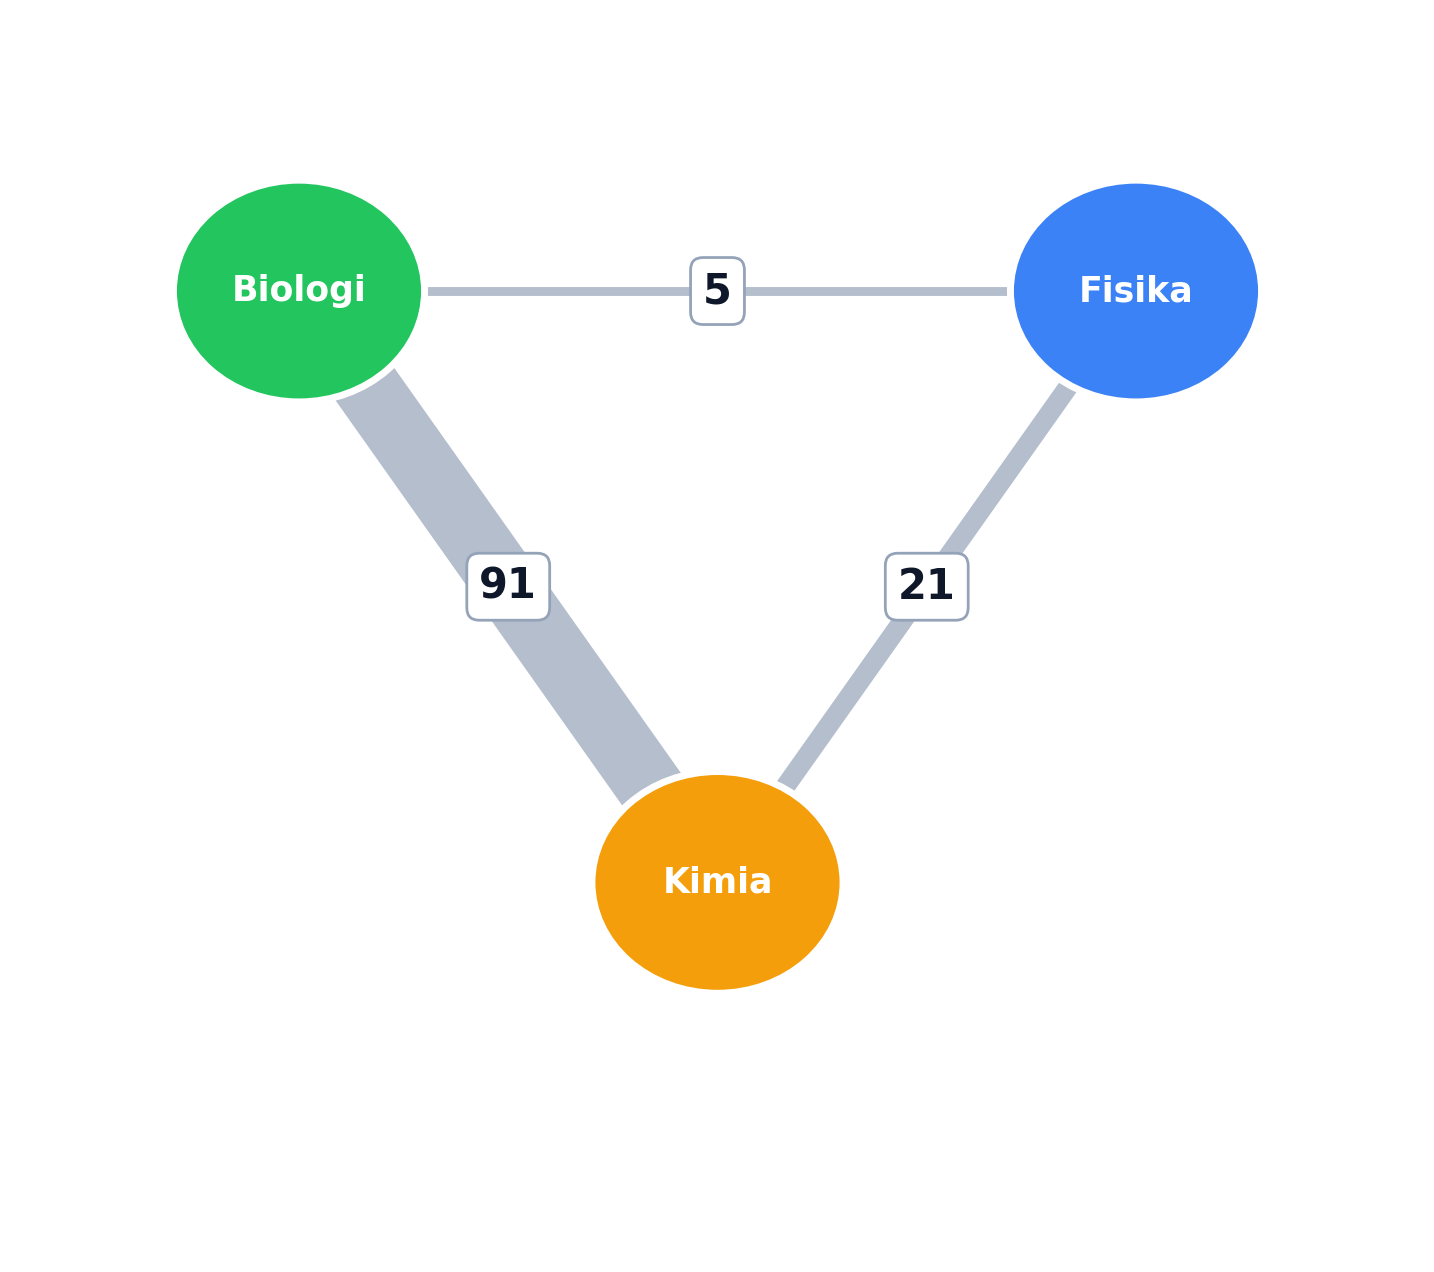
\includegraphics[width=0.85\linewidth]{images/media/image14.png}
  \caption{\textit{Inter-domain bridge graph}. Setiap simpul adalah satu mata pelajaran;
    ketebalan dan label sisi menyatakan jumlah relasi lintas-buku yang ditemukan
    antar pasangan disiplin (dari 117 relasi yang disurvei pada konfigurasi final).}
  \label{fig:bridge-graph}
\end{figure}

Distribusi jembatan lintas-disiplin sangat tidak merata. Pasangan
Biologi--Kimia mendominasi (91 relasi, 78\%), diikuti Fisika--Kimia (21
relasi, 18\%), sedangkan Biologi--Fisika nyaris tidak terhubung (5
relasi, 4\%). Pola ini menempatkan Kimia sebagai poros (\textit{hub}) yang
menjembatani kedua disiplin lain. Temuan ini konsisten secara pedagogis:
tumpang-tindih molekuler dan biokimiawi (DNA, protein, enzim, reaksi
redoks) membuat Biologi dan Kimia berbagi banyak konsep dasar, sementara
keterkaitan Fisika sebagian besar terbatas pada elektrokimia (arus dan
potensial listrik $\leftrightarrow$ sel elektrokimia). Sifat Fisika yang lebih
abstrak-matematis menjadikannya domain paling terisolasi dalam jaringan
konsep kurikulum kelas XII.

Dari sisi kualitas ekstraksi (validasi Fase 1), terdapat perbedaan
antar-domain:

\begin{longtable}{@{}
  >{\raggedright\arraybackslash}p{0.15\linewidth}
  >{\raggedright\arraybackslash}p{0.50\linewidth}
  >{\raggedright\arraybackslash}p{0.30\linewidth}@{}}
\caption{Presisi ekstraksi per domain sains (Fase 1 validasi pakar).}
\label{tab:komparatif-domain}\\
\toprule
\textbf{Domain} & \textbf{Presisi ekstraksi (Fase 1)} & \textbf{Catatan} \\
\midrule
\endhead
Biologi & $\sim$0{,}95--0{,}97 & paling konsisten; konsep deskriptif-naratif \\
Fisika  & $\sim$0{,}86--0{,}99 & rentang lebar; lemah pada relasi kuantitatif/rumus \\
Kimia   & $\sim$0{,}82--0{,}92 & kesalahan terbanyak pada terminologi proses \\
\bottomrule
\end{longtable}

Perbedaan ini selaras dengan analisis kesalahan pada Subbab~\ref{subsubsec:error-analysis}:
kelemahan utama pada Fisika adalah \textbf{\textit{under-extraction} rumus} (67\%
\textit{missing triples} Fisika berupa formula), sedangkan Kimia rentan pada
\textbf{pencampuran konsep teknis}. Biologi---yang materinya lebih
bersifat deskriptif---paling sesuai dengan kekuatan LLM dalam mengekstrak
struktur konseptual.

\ifSubfilesClassLoaded{\printbibliography[title={Daftar Pustaka}]}{}

\end{document}
